\section{System Architecture}
\label{sec:system_architecture}

The system follows a modular architecture that separates hardware configuration, servo communication, kinematic computation, feedback control, and distance sensing. The STM32U545 acts as the central embedded platform and executes the complete robot-side motion stack. It communicates with the daisy-chained Feetech servos through a serial bus driver board, while an ESP32 provides the interface to the external wireless sensing subsystem. Figure~\ref{fig:system_architecture} summarizes the resulting information and control flow.

\begin{figure}[!h]
    \centering
    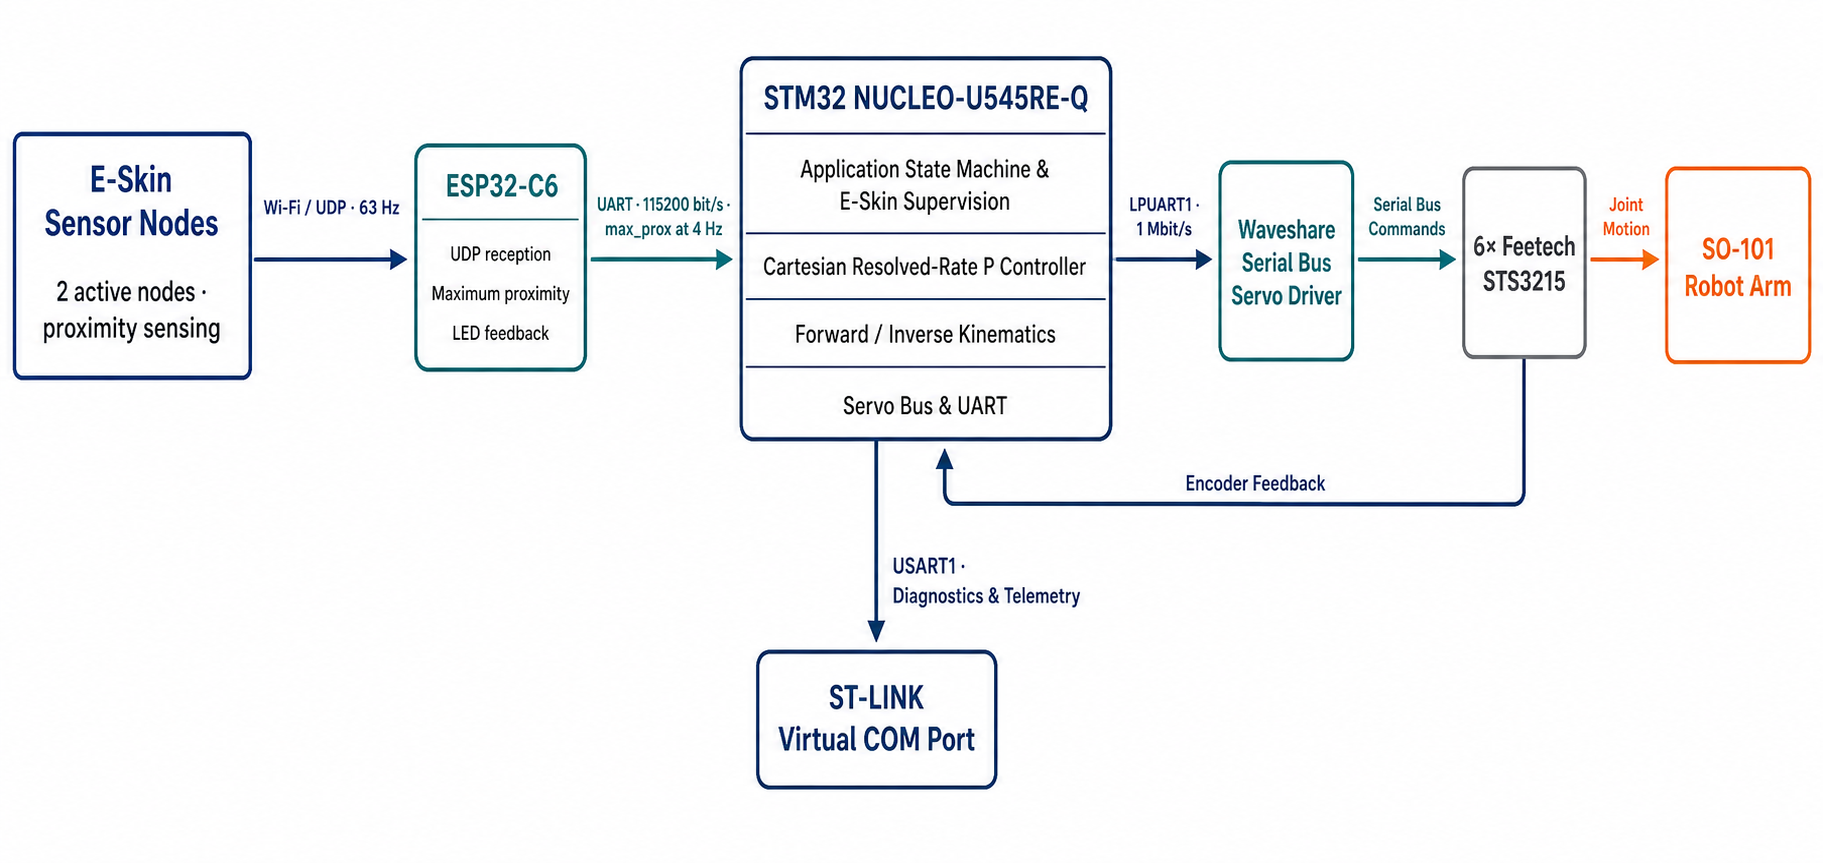
\includegraphics[width=\columnwidth]{figures/system_architecture.png}
    \caption{System architecture and information flow between the E-Skin sensors, ESP32, STM32, servo bus, and SO-101 robot arm. Own illustration, created with assistance from ChatGPT and manually revised by the authors.}
    \label{fig:system_architecture}
\end{figure}

The application is organized as a modular embedded architecture that separates motion control, kinematic computation, servo communication, and collision sensing. Cartesian motion requests are processed by the STM32-based control stack, while an independent ESP32-based sensing subsystem acquires wireless E-Skin measurements and provides collision-relevant feedback through a dedicated UART interface.

The technical contributions follow the dependencies of the complete system. Alessandro Canalicchio implemented the STM32 configuration, peripheral setup, firmware architecture, and integration of the application modules. Niklas Peter implemented the Feetech communication layer, servo abstraction, joint limits, forward and inverse kinematics, blocking and non-blocking motion interfaces, and computational benchmarks. The resulting joint targets are used by the feedback controller implemented by Alessandro Canalicchio. Emile Gebrael implemented the wireless distance-sensing interface, ESP32 signal processing, and collision-feedback logic. This separation enabled the individual components to be developed and tested independently before their integration into the final proof-of-concept system.

